\documentclass[11pt,a4paper]{article}

% =================================================================
%  Question Bank -- Unit IV: Introduction to Robotics
%  Self-contained: all block diagrams / flowcharts drawn with TikZ.
% =================================================================

\usepackage[margin=2cm, headheight=14pt]{geometry}
\usepackage{amsmath}
\usepackage{amssymb}
\usepackage{bm}
\usepackage{array}
\usepackage{booktabs}
\usepackage{enumitem}
\usepackage{xcolor}
\usepackage{tikz}
\usepackage[most]{tcolorbox}
\usepackage{fancyhdr}
\usepackage{helvet}
\renewcommand{\familydefault}{\sfdefault}
\setlength{\emergencystretch}{2em}

\usetikzlibrary{shapes.geometric, arrows.meta, positioning, calc, fit, backgrounds, patterns}

% -------------------------------------------------
% Colour palette (same as the lecture decks)
% -------------------------------------------------
\definecolor{cAccent}{RGB}{0,102,153}
\definecolor{cGreen}{RGB}{34,139,34}
\definecolor{cRed}{RGB}{178,34,34}
\definecolor{cOrange}{RGB}{204,102,0}
\definecolor{cPurple}{RGB}{102,45,145}
\definecolor{cGrayBg}{RGB}{245,246,248}

% -------------------------------------------------
% TikZ styles
% -------------------------------------------------
\tikzset{
	process/.style  ={rectangle, minimum width=2.6cm, minimum height=0.8cm, text centered, align=center, text width=2.6cm, draw=black, fill=blue!8},
	decision/.style ={diamond, aspect=2, minimum width=2.4cm, minimum height=0.9cm, text centered, text width=2.4cm, draw=black, fill=cGreen!18, inner sep=1pt},
	startstop/.style={rectangle, rounded corners=8pt, minimum width=2.2cm, minimum height=0.7cm, text centered, align=center, draw=black, fill=cAccent!25},
	flowarrow/.style={-{Stealth[length=2.5mm]}, thick},
	blk/.style      ={rectangle, draw=black, thick, minimum width=1.9cm, minimum height=0.9cm, align=center, fill=blue!8},
	sumj/.style     ={circle, draw=black, thick, minimum size=0.55cm, inner sep=0pt},
	sig/.style      ={-{Stealth[length=2.2mm]}, thick},
	vflow/.style    ={-{Stealth[length=2mm]}, thick},
}
% valve-symbol helpers
\newcommand{\vspring}[2]{%
	\draw[thick] (#1,#2) -- ++(0.08,0.18) -- ++(0.1,-0.36) -- ++(0.1,0.36) -- ++(0.1,-0.36) -- ++(0.1,0.36) -- ++(0.08,-0.18);}
\newcommand{\vsolenoid}[2]{%
	\draw[thick] ({#1-0.45},{#2-0.22}) rectangle (#1,{#2+0.22});
	\draw[thick] ({#1-0.45},{#2-0.22}) -- (#1,{#2+0.22});}
\newcommand{\vblock}[3]{%
	\draw[thick] (#1,#2) -- (#1,{#2+#3});
	\draw[thick] ({#1-0.12},{#2+#3}) -- ({#1+0.12},{#2+#3});}

% ladder-logic helpers
\newcommand{\ladNO}[3]{%
	\draw[thick] ({#1-0.15},{#2-0.25}) -- ({#1-0.15},{#2+0.25});
	\draw[thick] ({#1+0.15},{#2-0.25}) -- ({#1+0.15},{#2+0.25});
	\node[above=1pt, font=\scriptsize] at (#1,{#2+0.25}) {#3};}
\newcommand{\ladNC}[3]{%
	\ladNO{#1}{#2}{#3}
	\draw[thick] ({#1-0.25},{#2-0.3}) -- ({#1+0.25},{#2+0.3});}
\newcommand{\ladCoil}[3]{%
	\draw[thick] (#1,#2) circle (0.28);
	\node[above=1pt, font=\scriptsize] at (#1,{#2+0.28}) {#3};}

% -------------------------------------------------
% Question / answer layout
% -------------------------------------------------
\newcommand{\opts}[4]{%
	\par\smallskip
	\begin{tabular}{@{}p{0.46\linewidth}p{0.46\linewidth}@{}}
		(a) #1 & (b) #2 \\
		(c) #3 & (d) #4 \\
	\end{tabular}\par}
\newcommand{\ans}[1]{%
	\par\smallskip
	{\color{cGreen!50!black}\textbf{Answer:} #1}\par\medskip}
\newtcolorbox{answer}{breakable, enhanced, colback=cGreen!4, colframe=cGreen!55!black,
	boxrule=0.6pt, arc=2pt, left=6pt, right=6pt, top=4pt, bottom=4pt,
	title={Answer}, fonttitle=\bfseries\small, coltitle=white}
\newcommand{\qmarks}[1]{\hfill\textbf{[#1]}}
\newcommand{\partheading}[2]{%
	\bigskip
	\begin{tcolorbox}[colback=cAccent!10, colframe=cAccent, boxrule=0.6pt, arc=2pt, left=6pt, top=3pt, bottom=3pt]
		\textbf{\large #1} \hfill \textbf{#2}
	\end{tcolorbox}}

\setlist[enumerate,1]{label=\textbf{Q\arabic*.}, leftmargin=*, itemsep=6pt}

\pagestyle{fancy}
\fancyhf{}
\lhead{\small Question Bank --- Unit IV}
\rhead{\small Introduction to Robotics}
\cfoot{\small \thepage}

\begin{document}

	% -------------------------------------------------
	% Title block
	% -------------------------------------------------
	\begin{center}
		{\Large\bfseries\color{cAccent} Question Bank}\\[4pt]
		{\large\bfseries Unit IV: Introduction to Robotics}\quad(12 Hrs.)\\[6pt]
		{\small Amit Kumar Singh, Assistant Professor (ECE), School of Naval Architecture and Ocean Engineering\\
			Indian Maritime University, Visakhapatnam Campus}
	\end{center}

	\noindent\textbf{Syllabus:} Introduction to robotics: synthesis of elements with movability constraints; elements of robot anatomy; hydraulic, pneumatic and electrical manipulators; end-effectors and their design; controllers with microprocessors or fluidics; robot sensors; applications of industrial robots; economics of robotics.

	\medskip
	\noindent
	\begin{tabular}{@{}lll@{}}
		\textbf{Part A} & 10 multiple-choice questions & $10\times1 = 10$ marks \\
		\textbf{Part B} & 5 short-answer questions      & $5\times2 = 10$ marks \\
		\textbf{Part C} & 3 long-answer questions       & $3\times10 = 30$ marks \\
	\end{tabular}

	% =================================================================
	\partheading{Part A: Multiple-Choice Questions}{1 mark each}
	% =================================================================
	\begin{enumerate}

		\item A robot whose arm has three linear (sliding) joints is called
		\opts{Cylindrical}{Cartesian}{Polar}{Articulated}
		\ans{(b) Cartesian (gantry) --- LOO joints, box-shaped work envelope.}

		\item SCARA stands for
		\opts{Simple Compliant Automatic Robot Arm}{Sensor Controlled Assembly Robot Arm}{Serial Controlled Articulated Robot Arm}{Selective Compliance Assembly Robot Arm}
		\ans{(d) Selective Compliance Assembly Robot Arm.}

		\item A free rigid body in space has how many degrees of freedom?
		\opts{3}{4}{6}{12}
		\ans{(c) 6 --- three translations and three rotations.}

		\item A revolute (R) joint provides how many degrees of freedom?
		\opts{1}{0}{2}{3}
		\ans{(a) 1 --- rotation about one axis.}

		\item A gripper that lifts flat glass sheets by suction is a
		\opts{magnetic gripper}{hook}{mechanical gripper}{vacuum gripper}
		\ans{(d) Vacuum gripper (suction cups).}

		\item The sensor most commonly used to measure robot joint position is the
		\opts{thermocouple}{encoder}{strain gauge}{microphone}
		\ans{(b) Encoder (incremental or absolute).}

		\item The first industrial robot, installed at General Motors in 1961, was
		\opts{PUMA}{SCARA}{Unimate}{ASIMO}
		\ans{(c) Unimate (hydraulically driven).}

		\item Fluidic logic controllers use
		\opts{jets of air or liquid}{transistors}{optical fibres}{relays}
		\ans{(a) Jets of air or liquid, with no moving parts (Coanda / wall-attachment effect).}

		\item Which drive system gives the highest payload capacity?
		\opts{Pneumatic}{Solenoid}{Stepper motor}{Hydraulic}
		\ans{(d) Hydraulic.}

		\item The work envelope of a cylindrical robot is shaped like a
		\opts{box}{hollow cylinder}{sphere}{cone}
		\ans{(b) Hollow cylinder (portion of an annular cylinder).}

	\end{enumerate}

	% =================================================================
	\partheading{Part B: Short-Answer Questions}{2 marks each}
	% =================================================================
	\begin{enumerate}

		\item State the Gr\"ubler--Kutzbach mobility equation for planar mechanisms and find the mobility of a four-bar linkage. \qmarks{2}
		\begin{answer}
			$M = 3(n-1) - 2j_1 - j_2$, where $n$ = number of links (including the fixed link), $j_1$ = 1-DOF joints, $j_2$ = 2-DOF joints.\\
			Four-bar: $n = 4$, $j_1 = 4$ $\Rightarrow$ $M = 3(3) - 2(4) = \mathbf{1}$ --- one input (motor) drives it.
		\end{answer}

		\item Differentiate between accuracy and repeatability of a robot. \qmarks{2}
		\begin{answer}
			\textbf{Accuracy} is how closely the robot reaches a \emph{commanded} point in space: accuracy $= \text{CR}/2 + 3\sigma$. \textbf{Repeatability} is how closely it returns to a previously \emph{taught} point: $\pm3\sigma$. Robots are usually much more repeatable than accurate.
		\end{answer}

		\item A 2 kg part is held between two fingers with coefficient of friction 0.3. Find the gripping force needed to hold it at rest (take $g = 9.81$ m/s$^2$). \qmarks{2}
		\begin{answer}
			$\mu\,n_f\,F_g = m g \Rightarrow F_g = \dfrac{m g}{\mu n_f} = \dfrac{2\times9.81}{0.3\times2} = \mathbf{32.7\ N}$ (a safety factor, e.g.\ 2, is then applied).
		\end{answer}

		\item Distinguish between internal and external robot sensors, with two examples of each. \qmarks{2}
		\begin{answer}
			\textbf{Internal sensors} measure the robot's own state --- e.g.\ encoders (joint position), tachogenerators (joint velocity). \textbf{External sensors} measure the environment --- e.g.\ proximity sensors, force--torque sensors, vision cameras, touch sensors.
		\end{answer}

		\item A robot installation costs Rs 40 lakh and gives a net saving of Rs 12 lakh per year. Find the payback period and the return on investment. \qmarks{2}
		\begin{answer}
			Payback $= 40/12 \approx \mathbf{3.3\ years}$;\quad ROI $= 12/40\times100 = \mathbf{30\,\%}$ per year.
		\end{answer}

	\end{enumerate}

	% =================================================================
	\partheading{Part C: Long-Answer Questions}{10 marks each}
	% =================================================================
	\begin{enumerate}

		% -------------------------------------------------------------
		\item Explain the components of an industrial robot system with a block diagram. Describe the elements of robot anatomy and the five common robot configurations with their work envelopes and applications. \qmarks{10}
		\begin{answer}
			\textbf{(a) Robot system}
			\begin{center}
				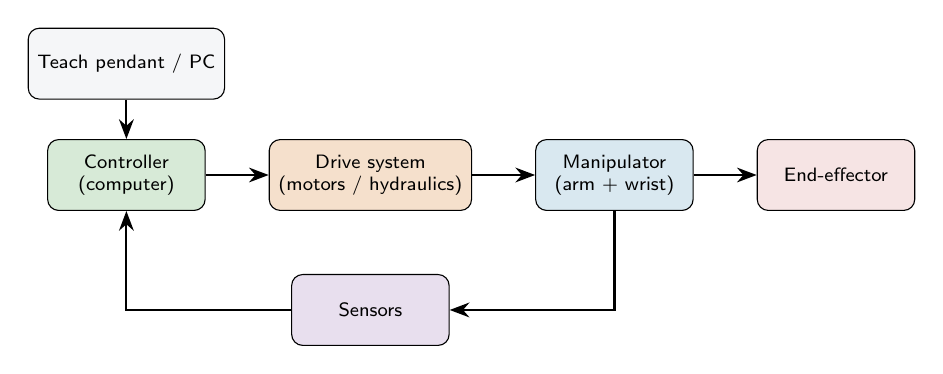
\begin{tikzpicture}[every node/.style={font=\scriptsize},
					el/.style={rectangle, draw=black, rounded corners, minimum width=2.0cm, minimum height=0.9cm, align=center, fill=blue!8}]
					\node[el, fill=cGreen!18] (ctrl) {Controller\\ (computer)};
					\node[el, right=0.8cm of ctrl, fill=cOrange!20] (drv) {Drive system\\ (motors / hydraulics)};
					\node[el, right=0.8cm of drv, fill=cAccent!15] (man) {Manipulator\\ (arm + wrist)};
					\node[el, right=0.8cm of man, fill=cRed!12] (ee) {End-effector};
					\node[el, below=0.8cm of drv, fill=cPurple!15] (sen) {Sensors};
					\node[el, above=0.5cm of ctrl, fill=cGrayBg] (tp) {Teach pendant / PC};
					\draw[flowarrow] (tp) -- (ctrl); \draw[flowarrow] (ctrl) -- (drv); \draw[flowarrow] (drv) -- (man); \draw[flowarrow] (man) -- (ee);
					\draw[flowarrow] (man.south) |- (sen.east); \draw[flowarrow] (sen.west) -| (ctrl.south);
				\end{tikzpicture}
			\end{center}
			The \textbf{controller} stores the program and plans the motion; the \textbf{drive system} powers the joints; the \textbf{manipulator} moves in space; the \textbf{end-effector} does the job; \textbf{sensors} feed back the arm position and information about the surroundings.

			\textbf{(b) Robot anatomy}
			\begin{itemize}[itemsep=1pt]
				\item \textbf{Base} --- fixed to floor, ceiling or a track.
				\item \textbf{Arm (body)} --- first three joints (waist, shoulder, elbow); \textbf{position} the wrist in space.
				\item \textbf{Wrist} --- last 2--3 joints (roll, pitch, yaw); \textbf{orient} the tool.
				\item \textbf{End-effector} --- gripper or tool on the wrist flange; the \textbf{tool centre point} is the point that is programmed.
				\item Joints: linear (L), orthogonal (O) --- prismatic; rotational (R), twisting (T), revolving (V) --- revolute.
			\end{itemize}

			\textbf{(c) Configurations}
			\begin{center}
				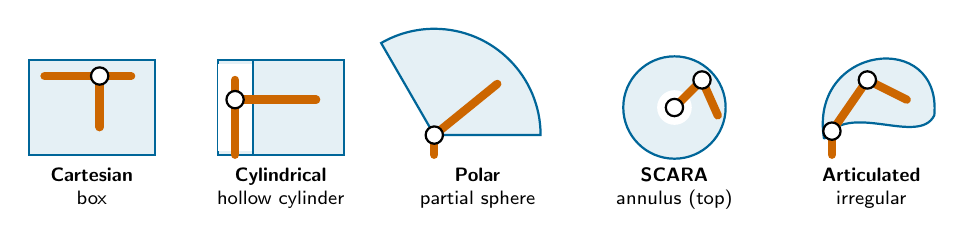
\begin{tikzpicture}[font=\scriptsize, link/.style={line width=3pt, cOrange, line cap=round},
					joint/.style={circle, draw=black, thick, fill=white, minimum size=0.22cm, inner sep=0pt}]
					\begin{scope}[shift={(0,0)}]
						\draw[thick, cAccent, fill=cAccent!10] (0,0) rectangle (1.6,1.2);
						\draw[link] (0.2,1.0) -- (1.3,1.0); \draw[link] (0.9,1.0) -- (0.9,0.35); \node[joint] at (0.9,1.0) {};
						\node[below, align=center] at (0.8,-0.05) {\textbf{Cartesian}\\ box};
					\end{scope}
					\begin{scope}[shift={(2.4,0)}]
						\draw[thick, cAccent, fill=cAccent!10] (0,0) rectangle (1.6,1.2); \fill[white] (0,0.05) rectangle (0.45,1.15);
						\draw[thick, cAccent] (0.45,0) -- (0.45,1.2);
						\draw[link] (0.22,0) -- (0.22,0.95); \draw[link] (0.22,0.7) -- (1.25,0.7); \node[joint] at (0.22,0.7) {};
						\node[below, align=center] at (0.8,-0.05) {\textbf{Cylindrical}\\ hollow cylinder};
					\end{scope}
					\begin{scope}[shift={(4.9,0)}]
						\filldraw[thick, cAccent, fill=cAccent!10] (0.25,0.25) -- (1.6,0.25) arc (0:120:1.35) -- cycle;
						\draw[link] (0.25,0) -- (0.25,0.25); \draw[link] (0.25,0.25) -- (1.05,0.9); \node[joint] at (0.25,0.25) {};
						\node[below, align=center] at (0.8,-0.05) {\textbf{Polar}\\ partial sphere};
					\end{scope}
					\begin{scope}[shift={(7.4,0)}]
						\filldraw[thick, cAccent, fill=cAccent!10] (0.8,0.6) circle (0.65); \fill[white] (0.8,0.6) circle (0.22);
						\draw[link] (0.8,0.6) -- (1.15,0.95); \draw[link] (1.15,0.95) -- (1.35,0.5);
						\node[joint] at (0.8,0.6) {}; \node[joint] at (1.15,0.95) {};
						\node[below, align=center] at (0.8,-0.05) {\textbf{SCARA}\\ annulus (top)};
					\end{scope}
					\begin{scope}[shift={(9.9,0)}]
						\filldraw[thick, cAccent, fill=cAccent!10] (0.2,0.2) .. controls (0.0,1.4) and (1.7,1.6) .. (1.6,0.5) .. controls (1.4,0.1) and (0.5,0.7) .. (0.2,0.2);
						\draw[link] (0.3,0) -- (0.3,0.3); \draw[link] (0.3,0.3) -- (0.75,0.95); \draw[link] (0.75,0.95) -- (1.25,0.7);
						\node[joint] at (0.3,0.3) {}; \node[joint] at (0.75,0.95) {};
						\node[below, align=center] at (0.8,-0.05) {\textbf{Articulated}\\ irregular};
					\end{scope}
				\end{tikzpicture}
			\end{center}
			\begin{center}
				\small
				\begin{tabular}{@{}llll@{}}
					\toprule
					\textbf{Configuration} & \textbf{Joints} & \textbf{Feature} & \textbf{Application} \\
					\midrule
					Cartesian   & LOO & rigid, accurate          & gantry loading, palletising \\
					Cylindrical & TLO & large vertical reach     & machine loading \\
					Polar       & TRL & long horizontal reach    & spot welding, die casting \\
					SCARA       & VRO & fast, stiff vertically   & electronic assembly \\
					Articulated & TRR & dexterous, compact       & arc welding, painting \\
					\bottomrule
				\end{tabular}
			\end{center}
		\end{answer}

		% -------------------------------------------------------------
		\item Classify end-effectors with a neat diagram. Explain the working of a mechanical gripper and derive the expression for the gripping force. Design a vacuum cup to lift a 5 kg plate at 60 kPa vacuum with a safety factor of 2. \qmarks{10}
		\begin{answer}
			\textbf{(a) Classification}
			\begin{center}
				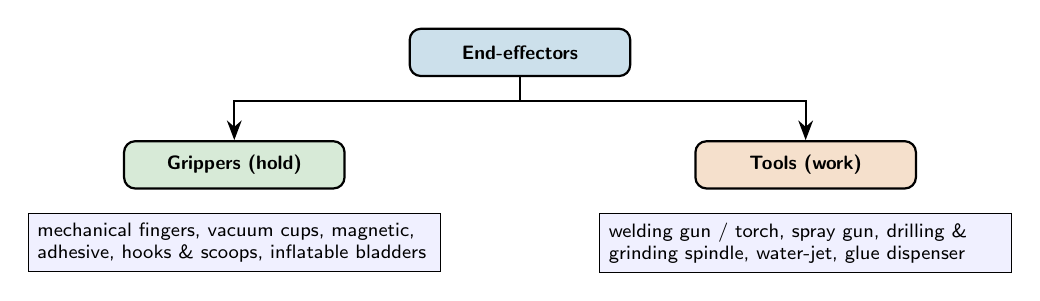
\begin{tikzpicture}[every node/.style={font=\scriptsize},
					hdr/.style={rectangle, draw=black, thick, rounded corners, minimum width=2.8cm, minimum height=0.6cm, align=center, font=\bfseries\scriptsize, fill=cAccent!20},
					grp/.style={rectangle, draw=black, align=left, fill=blue!6, text width=5.0cm}]
					\node[hdr] (ee) {End-effectors};
					\node[hdr, below left=0.8cm and 0.8cm of ee, fill=cGreen!18] (gr) {Grippers (hold)};
					\node[hdr, below right=0.8cm and 0.8cm of ee, fill=cOrange!20] (tl) {Tools (work)};
					\draw[flowarrow] (ee.south) -- ++(0,-0.3) -| (gr.north);
					\draw[flowarrow] (ee.south) -- ++(0,-0.3) -| (tl.north);
					\node[grp, below=0.3cm of gr] {mechanical fingers, vacuum cups, magnetic, adhesive, hooks \& scoops, inflatable bladders};
					\node[grp, below=0.3cm of tl] {welding gun / torch, spray gun, drilling \& grinding spindle, water-jet, glue dispenser};
				\end{tikzpicture}
			\end{center}

			\noindent\begin{minipage}[t]{0.42\linewidth}
				\textbf{(b) Mechanical gripper}
				\begin{center}
					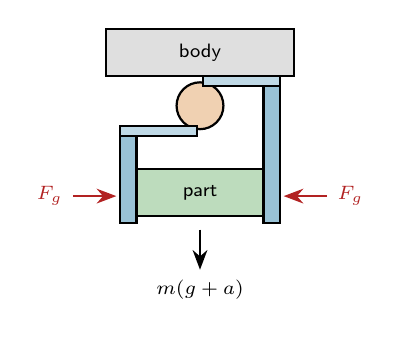
\begin{tikzpicture}[font=\scriptsize, scale=0.85]
						\filldraw[fill=gray!25, thick] (-1.4,1.8) rectangle (1.4,2.5);
						\node at (0,2.15) {body};
						\draw[thick, fill=cOrange!30] (0,1.35) circle (0.35);
						\filldraw[fill=cAccent!25, thick] (-1.2,0.9) rectangle (-0.05,1.05);
						\filldraw[fill=cAccent!25, thick] (0.05,1.65) rectangle (1.2,1.8);
						\filldraw[fill=cAccent!40, thick] (-1.2,0.9) rectangle (-0.95,-0.4);
						\filldraw[fill=cAccent!40, thick] (0.95,1.65) rectangle (1.2,-0.4);
						\filldraw[fill=cGreen!30, thick] (-0.95,-0.3) rectangle (0.95,0.4);
						\node at (0,0.05) {part};
						\draw[flowarrow, cRed] (-1.9,0.0) -- (-1.25,0.0) node[pos=0,left] {$F_g$};
						\draw[flowarrow, cRed] (1.9,0.0) -- (1.25,0.0) node[pos=0,right] {$F_g$};
						\draw[flowarrow] (0,-0.5) -- (0,-1.1) node[below] {$m(g+a)$};
					\end{tikzpicture}
				\end{center}
			\end{minipage}\hfill
			\begin{minipage}[t]{0.55\linewidth}
				A pneumatic cylinder or motor turns a pinion that moves two racks in opposite directions, so both fingers close equally on the part (rack-and-pinion parallel gripper). Other mechanisms: linkages (toggle), cams, screws.

				\smallskip
				\textbf{Gripping force:} the friction at all contact surfaces must support the weight and inertia force:
				\[
				\mu\,n_f\,F_g \ge m(g+a)
				\;\Rightarrow\;
				F_g = \frac{m(g+a)}{\mu\,n_f}\times\text{SF}
				\]
				$\mu$ = friction coefficient, $n_f$ = number of contact surfaces, $a$ = acceleration, SF = safety factor.

				\smallskip
				e.g.\ $m = 2$ kg, $\mu = 0.3$, $n_f = 2$, $a = 10$ m/s$^2$, SF $= 2$: $F_g = \dfrac{2(19.81)}{0.6}\times2 \approx 132$ N.
			\end{minipage}

			\medskip
			\textbf{(c) Vacuum cup design} ($m = 5$ kg, $\Delta p = 60$ kPa, SF $= 2$)
			\[
			A = \frac{\text{SF}\cdot m g}{\Delta p} = \frac{2\times5\times9.81}{60\,000} = 1.64\times10^{-3}\ \text{m}^2,
			\qquad
			D = \sqrt{\frac{4A}{\pi}} \approx \mathbf{46\ mm}
			\]
			A standard 50 mm cup would be chosen.

			\textbf{(d) Design considerations}: part mass, shape, surface and fragility; gripping method; end-effector weight (reduces payload); tolerance and need for compliance (RCC device); sensing (part-present switch); power supply (air, vacuum, electric); quick tool change.
		\end{answer}

		% -------------------------------------------------------------
		\item Explain the levels of robot control. With a block diagram, explain a microprocessor-based robot controller, and describe fluidic control. Compare microprocessor and fluidic controllers. \qmarks{10}
		\begin{answer}
			\textbf{(a) Levels of robot control}
			\begin{itemize}[itemsep=1pt]
				\item \textbf{Limited-sequence (bang-bang)} --- joints move between mechanical stops; sequence from a timer or logic (fluidics, PLC, cams).
				\item \textbf{Playback, point-to-point} --- taught points stored; the path between them is not controlled.
				\item \textbf{Playback, continuous path} --- the whole path (lines, arcs) is controlled by interpolation.
				\item \textbf{Intelligent} --- uses sensors and vision to change its actions; takes decisions.
			\end{itemize}

			\textbf{(b) Microprocessor-based controller}
			\begin{center}
				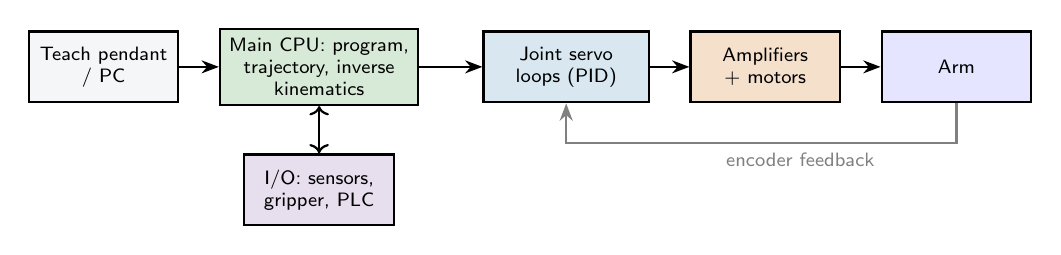
\begin{tikzpicture}[font=\scriptsize, node distance=0.5cm]
					\node[blk, fill=cGrayBg] (tp) {Teach pendant\\ / PC};
					\node[blk, right=of tp, fill=cGreen!18, minimum width=2.4cm] (cpu) {Main CPU: program,\\ trajectory, inverse\\ kinematics};
					\node[blk, right=0.8cm of cpu, fill=cAccent!15, minimum width=2.1cm] (j1) {Joint servo\\ loops (PID)};
					\node[blk, right=of j1, fill=cOrange!20] (amp) {Amplifiers\\ + motors};
					\node[blk, right=of amp, fill=blue!10] (arm) {Arm};
					\node[blk, below=0.6cm of cpu, fill=cPurple!15] (io) {I/O: sensors,\\ gripper, PLC};
					\draw[sig] (tp) -- (cpu); \draw[sig] (cpu) -- (j1); \draw[sig] (j1) -- (amp); \draw[sig] (amp) -- (arm);
					\draw[sig, gray] (arm.south) -- ++(0,-0.5) -| node[pos=0.2, below] {encoder feedback} (j1.south);
					\draw[<->, thick] (cpu) -- (io);
				\end{tikzpicture}
			\end{center}
			The \textbf{main processor} interprets the program, plans the path and solves the inverse kinematics every few milliseconds. \textbf{Joint processors} run a PID position loop for each joint at 1--10 kHz using encoder feedback. The \textbf{I/O} section handles grippers, conveyors, machine tools and safety interlocks. Programs are entered by teach pendant, lead-through or off-line programming.

			\textbf{(c) Fluidic control}: logic elements made of channels in which a \textbf{jet of air} attaches to one wall (Coanda effect); a small control jet switches it to the other outlet --- a binary element with \textbf{no moving parts}. AND, OR, NOT, NOR, flip-flops and timers can be built and connected directly to pneumatic cylinders, making simple \textbf{limited-sequence pick-and-place robots}.

			\textbf{(d) Comparison}
			\begin{center}
				\small
				\begin{tabular}{@{}p{3.0cm}p{5.4cm}p{5.4cm}@{}}
					\toprule
					\textbf{Feature} & \textbf{Microprocessor} & \textbf{Fluidic} \\
					\midrule
					Signal      & electrical bits            & air-jet pressure (0/1) \\
					Speed       & microseconds               & milliseconds \\
					Functions   & arithmetic, kinematics, PID, vision & ON/OFF logic and sequencing only \\
					Programming & software, easy to change   & re-plumb the circuit \\
					Environment & needs protection from heat, EMI, sparks & safe in explosive, hot, radioactive areas \\
					Typical use & servo, continuous-path, intelligent robots & limited-sequence pneumatic robots \\
					\bottomrule
				\end{tabular}
			\end{center}
		\end{answer}

	\end{enumerate}

\end{document}
